%!TEX encoding = UTF-8 Unicode
%!TEX root = ../lect-w05.tex

%%%

\ifkompendium\else

\Subsection{Veckans uppgifter}
\begin{SlideExtra}{Övning: \texttt{classes}}
\begin{itemize}\SlideFontSmall
%!TEX encoding = UTF-8 Unicode

%!TEX root = ../compendium1.tex

\item Kunna deklarera klasser med klassparametrar.
\item Kunna skapa instanser med \code{new}.
\item Kunna ge argument vid instansiering.
\item Förstå innebörden av referensvariabler och värdet \code{null}.

\item Kunna använda nyckelordet \code{private} för att styra synlighet av attribut och konstruktorparametrar.

\item Förstå syftet med getters och setters.
\item Kunna förklara accessregler för kompanjonsobjekt.
\item Kunna skapa fabriksmetod i kompanjonsobjekt.
\item Känna till nyttan med en privat konstruktor.

%\item Kunna implementera en klass utifrån en specifikation.
\item Förstå skillnaden mellan referenslikhet och strukturlikhet.
\item Känna till skillnaden mellan \code{==} och \code{eq}, samt \code{!=} och \code{ne}.

\item Kunna förklara hur case-klasser hanterar instansiering.
\item Känna till hur case-klasser hanterar likhet.

\end{itemize}
\end{SlideExtra}

\begin{SlideExtra}{Laboration: \texttt{blockbattle} redovisas NÄSTA vecka}
  \begin{minipage}{0.42\textwidth}
        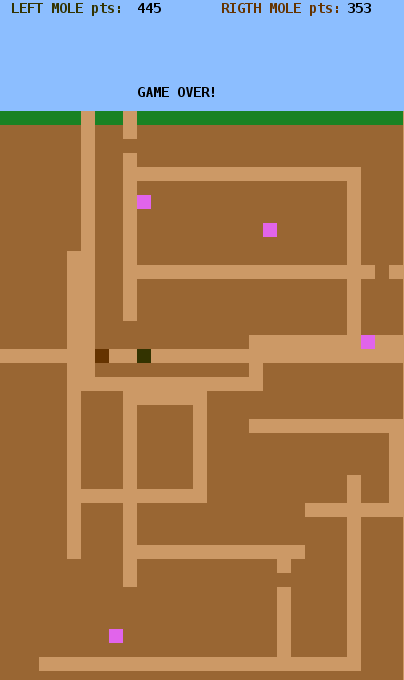
\includegraphics[height=0.8\textheight]{../img/blockbattle.png}
  \end{minipage}%
  \begin{minipage}{0.59\textwidth}
    \begin{itemize}
      \item Ett arkadspel för två spelare.
      \item Nu med TVÅ blockmullvader!
      \item Träna på att skapa och använda klasser för att möjliggöra flera instanser.
      \item Träna på att använda matchning.
      \item Programmet är väsentligt mer omfattande jämfört med tidigare laborationer.
      \item Du till nästa fredag på dig innan du ska redovisa.
    \end{itemize}    
  \end{minipage}
\end{SlideExtra}
  
\fi
